\documentclass[russian,utf8,emptystyle,reduceheight=5mm]{eskdtext}

% packages
%
% Тестовое наполнение текстом
% При написании работы - удалить пакет и комманды \lipsum
\usepackage{lipsum}
%
\usepackage{eskdplain}
\usepackage{graphicx}
\usepackage{datetime}
\usepackage{enumitem} % for lists
\usepackage{ulem} % for underlining
\usepackage{lastpage} % Number of pages
\usepackage{hyperref} % Links in pdf

% setup
\newcommand{\FrontPageDepartment}{ЭМ} %Факультет
\newcommand{\FrontPageSubdepartment}{Менеджмента} %Кафедра
\newcommand{\WorkType}{Контрольная работа} %Тип работы (заголовок)
\newcommand{\Subject}{Предмет} %по ... родительный падеж
\newcommand{\Topic}{Тема контрольной работы} %Тема
\newcommand{\Professor}{Иванов~И.~И.} %Руководитель
\newcommand{\Student}{Петров~П.~П.} %Студент
\newcommand{\Group}{ИСм-112} %Группа
\newcommand{\FrontPageDate}{\ddmmyyyydate\today} %Дата

\ESKDsignature{МИВУ 230400.68 ПЗ} % Код специальности и тип работы

% eskdx setup
\ESKDletter{}{У}{}
\ESKDtitle{\Topic}
\ESKDchecker{\Professor}
\ESKDauthor{\Student}
\ESKDcolumnIX{МИ ВлГУ\\ \Group}

\addto\captionsrussian{\def\refname{Список использованных источников}}
\sloppy % split long lines

% graphics path
\graphicspath{{src/img/}}

% verbatim setup
\newcommand{\verbatimFont}{
\fontsize{10pt}{12pt}\selectfont
\baselineskip=1em
}

% workaround for regression in babel package on linux
\newcommand{\No}{\textnumero}

% paragraph indent
\setlength{\parindent}{1.25cm}

% % % % % % % % % % % % % % % % % % % % % % % % % % % % % % % % % % % % % % % %

% lists
\setlist{nolistsep} % No vertical spaces between items in lists
\renewcommand{\alph}[1]{\asbuk{#1}} % cyrillic numbering (letters)
\setenumerate[1]{label=\alph*), fullwidth, itemindent=\parindent,
  listparindent=\parindent}
\setenumerate[2]{label=\arabic*), fullwidth, itemindent=\parindent,
  listparindent=\parindent, leftmargin=\parindent}

% % % % % % % % % % % % % % % % % % % % % % % % % % % % % % % % % % % % % % % %

% titles
\titleformat{\chapter}[block]
  {\indent\indent\bfseries}{\MakeUppercase{\chaptertitlename}\ \thechapter}{1ex}{\filright\MakeUppercase}
\titleformat{\section}[block]{\indent\indent\bfseries}{\thesection}{1ex}{\filright}
\titleformat{\subsection}[block]{\indent\indent}{\thesubsection}{1ex}{\filright}
\titleformat{\subsubsection}[block]{\indent\indent}{\thesubsubsection}{1ex}{\filright}

\titlespacing*{\chapter}{0pt}{0pt}{1em}
%\titlespacing*{\section}{0pt}{1em}{1em}
%\titlespacing*{\subsection}{0pt}{1em}{1ex}
%\titlespacing*{\subsubsection}{0pt}{1em}{1ex}

\newcommand{\MakeUppercasePdf}[1]{\texorpdfstring{\MakeUppercase{#1}}{#1}}

\makeatletter
\newcommand{\Chapter}{\@ifstar\@sChapter\@Chapter}
%
\newcommand{\@sChapter}[1]{
  \chapter*{\MakeUppercase{#1}}
  \addcontentsline{toc}{chapter}{\MakeUppercasePdf{#1}}
}
%
\newcommand{\@Chapter}[1]{
  \stepcounter{chapter}
  \chapter*{\MakeUppercase{\chaptertitlename}\ \thechapter\ \MakeUppercase{#1}}
  \addcontentsline{toc}{chapter}{\MakeUppercasePdf{\chaptertitlename}\ \thechapter\ \MakeUppercasePdf{#1}}
}
\makeatother

% % % % % % % % % % % % % % % % % % % % % % % % % % % % % % % % % % % % % % % %

% table of contents
\addto{\captionsrussian}{\renewcommand*{\contentsname}{\ContentsName}}
% contents name
\setlength{\cftbeforetoctitleskip}{0pt}
\setlength{\cftaftertoctitleskip}{0pt}
\renewcommand{\cfttoctitlefont}{\hfil\MakeUppercase}
\renewcommand{\cftaftertoctitle}{\hfil}
% for chapters
\renewcommand{\cftchapleader}{\cftdotfill{\cftdotsep}}
\renewcommand{\cftchapfont}{}
\setlength{\cftbeforechapskip}{0pt}
\renewcommand{\cftchappagefont}{}
\cftsetindents{chapter}{0em}{0em}
\setlength{\cftchapindent}{0pt}
% no hyphenation
\makeatletter
\renewcommand{\@tocrmarg}{2.55em plus1fil}
\makeatother

% % % % % % % % % % % % % % % % % % % % % % % % % % % % % % % % % % % % % % % %

% figures
\renewcommand{\thefigure}{\arabic{figure}} % numeration
\captionsetup[figure]{labelsep=endash,justification=centering}
\graphicspath{{\GraphicsPath}}

% % % % % % % % % % % % % % % % % % % % % % % % % % % % % % % % % % % % % % % %

% tables
\renewcommand{\thetable}{\arabic{table}} % numeration
\DeclareCaptionFormat{caption_table}{#1\\\centering{#3}}
\captionsetup[table]{format=caption_table,justification=raggedleft,singlelinecheck=false}

% % % % % % % % % % % % % % % % % % % % % % % % % % % % % % % % % % % % % % % %

% bibliography
\newenvironment{Bibliography}{}{}
\makeatletter
\@ifpackageloaded{biblatex}
{
  % BibLaTeX
  \expandafter\def\expandafter\BibliographyFile\expandafter{\BibliographyFile .bib}
  \addbibresource{\BibliographyFile}
  \defbibheading{bibliography}[\BibliographyName]{\Chapter*{#1}} % set bibliography name
  \defbibenvironment{bibliography} % set numerating of bibliography
  {\enumerate[label=\arabic*.,itemindent=\parindent]{}
  {\setlength{\leftmargin}{\bibhang}%
  \setlength{\itemindent}{-\leftmargin}%
  \setlength{\itemsep}{\bibitemsep}%
  \setlength{\parsep}{\bibparsep}}}
  {\endenumerate}
  {\item}
  %
  \renewcommand{\bibfont}{} % set same font as document
  \renewcommand{\mkgostheading}[1]{#1} % disable emphasing of title
  %
  \DeclareSortingScheme{SortATY}{ % custom sort by author, title, year (ATY)
    \sort{\field{author}}
    \sort{\field{title}}
    \sort{\field{year}}
  }
  \AtBeginEnvironment{Bibliography}{\printbibliography}
} % \@ifpackageloaded{biblatex} true
{ % \@ifpackageloaded{biblatex} false
% BibTex
  \addto{\captionsrussian}{\renewcommand*{\bibname}{\BibliographyName}}
  \settocbibname{\MakeUppercasePdf{\BibliographyName}}
  \makeatletter
  \renewcommand{\@biblabel}[1]{#1.}
  \makeatother

  \let\OLDthebibliography\thebibliography
  \renewcommand\thebibliography[1]{
    \OLDthebibliography{#1}
    \setlength{\parskip}{0pt}
    \setlength{\itemsep}{0pt plus 0.3ex}
  }
  \AtBeginEnvironment{Bibliography}{
    \bibliographystyle{ugost2008s}
    \bibliography{\BibliographyFile}
  }
} % \@ifpackageloaded{biblatex} false
\makeatother
% % % % % % % % % % % % % % % % % % % % % % % % % % % % % % % % % % % % % % % %

% Do not overfill text lines (instead of \sloppy)
\pretolerance 150
\tolerance 1414
\hbadness 1414
\emergencystretch 1.5em
\hfuzz 0.3pt
%\clubpenalty=10000
\widowpenalty=10000
\vfuzz \hfuzz
\raggedbottom
%

% main document
\begin{document}
% Титул
\ESKDthisStyle{empty}
\setlength{\topskip}{15pt}
\newlength{\frontpagefk} % Ширина поля Факультет/Кафедра
\setlength{\frontpagefk}{6cm}
\newlength{\frontpagerb} % Ширина надписей Руководитель/Студент и пр. под темой
\setlength{\frontpagerb}{6cm}
\newlength{\frontpagerbspace} % ??? (do not remove)
\setlength{\frontpagerbspace}{1cm}
\newlength{\FrontPageSubjSpace} % Ширина пробела до и после названия предмета
\setlength{\FrontPageSubjSpace}{1cm}
\newlength{\FrontPageTopicSpace} % Ширина пробела до и после темы
\setlength{\FrontPageTopicSpace}{0.5cm}

\thispagestyle{empty}
\begin{center}
{
\vspace*{-1.5cm}
\baselineskip=1.3em
{\small Министерство образования и науки Российской Федерации}\\
\textbf{Муромский институт (филиал)}\\
{\footnotesize федерального государственного бюджетного образовательного учреждения\\
высшего профессионального образования}\\
\textbf{<<Владимирский государственный университет\\
имени Александра Григорьевича и Николая Григорьевича\\
Столетовых>>\\
(МИ (филиал) ВлГУ)\\}
}

\bigskip
\begin{tabular}{l c}
\textbf{Факультет}&\underline{\makebox[\frontpagefk]{\FrontPageDepartment}}\\
\textbf{Кафедра}&\underline{\makebox[\frontpagefk]{\FrontPageSubdepartment}}\\
\end{tabular}

\vspace{\fill}
\begin{Huge}
\textbf{\textsl{\WorkType}}
\end{Huge}

\vspace{\fill}
по\underline{\makebox[\FrontPageSubjSpace]{}\Subject\makebox[\FrontPageSubjSpace]{}}

\smallskip
Тема:\underline{\makebox[\FrontPageTopicSpace]{}\Topic\makebox[\FrontPageTopicSpace]{}}

\vspace{\fill}

\begin{flushright}
\makebox[\frontpagerb][c]{
\makebox[\frontpagerb][l]{Руководитель}\hspace{\frontpagerbspace}}

\smallskip
\makebox[\frontpagerb][c]{
\raisebox{-\baselineskip}{\shortstack{\underline{\makebox[\frontpagerb][l]{\Professor}}\\
\begin{footnotesize}
(фамилия, инициалы)
\end{footnotesize}}}\hspace{\frontpagerbspace}}

\bigskip
\makebox[\frontpagerb][c]{
\raisebox{-\baselineskip}{\shortstack{\underline{\makebox[\frontpagerb][l]{}}\\
\begin{footnotesize}
(подпись)\hfill(дата)
\end{footnotesize}}}\hspace{\frontpagerbspace}}

\newcommand{\frontpagerbstudent}[2]{ %
\makebox[\frontpagerb]{ %
\raisebox{-\baselineskip}{\shortstack{#1\ \underline{\makebox[\frontpagerb-\widthof{#1\ }][c]{#2}}\\
\begin{footnotesize}
\makebox[\widthof{#1\ }][c]{}\makebox[\frontpagerb-\widthof{#1\ }][c]{(группа)}
\end{footnotesize}}}\hspace{\frontpagerbspace}}
}

\bigskip
\makebox[\frontpagerb][c]{\frontpagerbstudent{Студент}{\Group}}

\smallskip
\makebox[\frontpagerb][c]{
\raisebox{-\baselineskip}{\shortstack{\underline{\makebox[\frontpagerb][l]{\Student}}\\
\begin{footnotesize}
(фамилия, инициалы)
\end{footnotesize}}}\hspace{\frontpagerbspace}}

\renewcommand{\dateseparator}{.}

\bigskip
\makebox[\frontpagerb][c]{
\raisebox{-\baselineskip}{\shortstack{\underline{\makebox[\frontpagerb][r]{\FrontPageDate}}\\
\begin{footnotesize}
(подпись)\hfill(дата)
\end{footnotesize}}}\hspace{\frontpagerbspace}}

\end{flushright}

\vspace{\fill}
Муром \the\year
\vspace*{-1cm}
\end{center}
\setlength{\topskip}{0pt}
\newpage

% Аннотация
\ESKDthisStyle{empty}
\vspace*{\fill}
�������� ������ �������� ���������� � ���������� ...

� �������� ������� �������� ������� ����������� �������, ��������� ���������� ����������, ���������, �������� �����������, ������������ ������������ �������.

����� ������������� ������� ���������� \pageref{LastPage} ������. ���������� �������� - 2 �����. ������� �����������.
\vspace*{\fill}
\newpage

% Содержание
\setcounter{page}{4}
\tableofcontents
\newpage

% Основной текст
\section*{Введение}
\addcontentsline{toc}{section}{Введение}
\lipsum[1-3]
\clearpage



\section{Анализ технического задания}
\subsection{Постановка задачи}
\lipsum[4]

Пример библиографической ссылки~\cite{wiki_main}.
Пример нумерации:
\begin{enumerate}
\item пункт1;
\item пункт2;
\item пункт3;
\item пункт4;
\item пункт5;
\item пункт6;
\item пункт7.
\end{enumerate}

\lipsum[5]
\begin{itemize}
\item пункт1;
\item пункт2;
\item пункт3;
\item пункт4;
\item пункт5;
\item пункт6;
\item пункт7.
\end{itemize}

\subsection{Назначение разрабатываемого программного продукта}
\lipsum[6]

\subsection{Анализ исходных данных к курсовой работе}
\lipsum[7]

\subsection{Методы и алгоритмы решения задачи}
\lipsum[34]

\subsection{Требования к разработке}
\lipsum[38]
\clearpage



\section{Разработка математической модели}
\lipsum[40]
\clearpage



\section{Разработка алгоритмов работы системы}
\subsection{пункт1}
\lipsum[9]

\subsection{пункт2}
\lipsum[10]

\subsubsection{под под пункт 1}
\lipsum[11]

\subsubsection{под под пункт 2}
\lipsum[12]
\clearpage



\clearpage
\section{Разработка программной системы}
\subsection{пункт 1}
\lipsum[52]

\subsection{пункт 2}
Пример вставки исходного кода "как есть".
{\verbatimFont
\begin{verbatim}
#include <iostream>

int main()
{
    std::cout << "Hello, World!";
}
\end{verbatim}}

\lipsum[13]
\clearpage



\section{Руководство по программному продукту}
\subsection{Руководство программиста}
Структура проекта представлена на рисунке~\ref{fig:structure} (пример вставки рисунка).

\begin{figure}[!h]
\centering
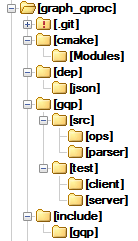
\includegraphics[scale=1]{structure}
\caption{Дерево файлов проекта}
\label{fig:structure}
\end{figure}

\lipsum[14-16]

\subsection{Руководство администратора}
\lipsum[17]

\subsection{Руководство пользователя}
\lipsum[18-19]
\newpage



\section{Тестирование системы}
\lipsum[19-21]
\clearpage



\section*{Заключение}
%\addtocontents{toc}{\protect\clearpage}
\addcontentsline{toc}{section}{Заключение}
\lipsum[23-25]
\newpage

% Список литературы
\begin{thebibliography}{00}

\bibitem{bib_name1} �������� 1

\bibitem{bib_name2} �������� 2

\bibitem{bib_name3} �������� 3

\bibitem{wiki_main} ���������: ��������� ������������: �� ������� ����� [����������� ������] // URL:  http://ru.wikipedia.org/wiki/���������\_��������  (���� ���������: 06.05.2013)

\bibitem{wiki_main} ���������: ��������� ������������: �� ������� ����� [����������� ������] // URL:  http://ru.wikipedia.org/wiki/���������\_��������  (���� ���������: \ddmmyyyydate\today)

\end{thebibliography}
\end{document}